\documentclass[9pt,onecolumn,twoside]{pnas-new}
% Remove the twocolumn option to create a single column SI file if required.
% Use the lineno option to display guide line numbers if required.
% Note that the use of elements such as single-column equations
% may affect the guide line number alignment.

\templatetype{pnassupportinginfo}
\usepackage{listings}
\lstset{basicstyle=\ttfamily,
  showstringspaces=false,
  commentstyle=\color{red},
  keywordstyle=\color{blue}
}
\title{Supporting Information}
\author{Hough et al.}

\doi{genetics.XXXXXXXXXX}

\begin{document}

\maketitle

%\section*{Supporting Information (SI)}

%All supporting information can be obtained from https://github.com/houghjosh/XYdiversity.

\section*{SI Tables}

\begin{table}[tbhp!]
\centering
\caption{Population identities (ID) and location information for \textit{R. hastatulus} samples}
\begin{tabular}{lllll}
Population ID & Location & Altitude & Latitude & Longitude \\
\midrule
\textbf{Texas} &  &  &  &  \\
TX-MTP & Mount Pleasant, Texas & 130	 & 33.17453 & 94.98799 \\
OK-RAT & Rattan, Oklahoma & 138 & 34.15755 & 95.41325 \\
TX-LIV & Livingston, Texas & 83 & 30.69947 & 94.79981 \\
LA-DER & De Ridder, Lousiana & 67 & 30.8941 & 93.3143 \\
TX-ATH & Athens, Texas & 145 & 32.18471 & 95.8032 \\
OK-WIL & Willis, Oklahoma & 211 & 33.89663 & 96.83533 \\
\bottomrule
\end{tabular}
\end{table}

\section*{SI Figures}

\begin{figure}[tbhp!]
\centering
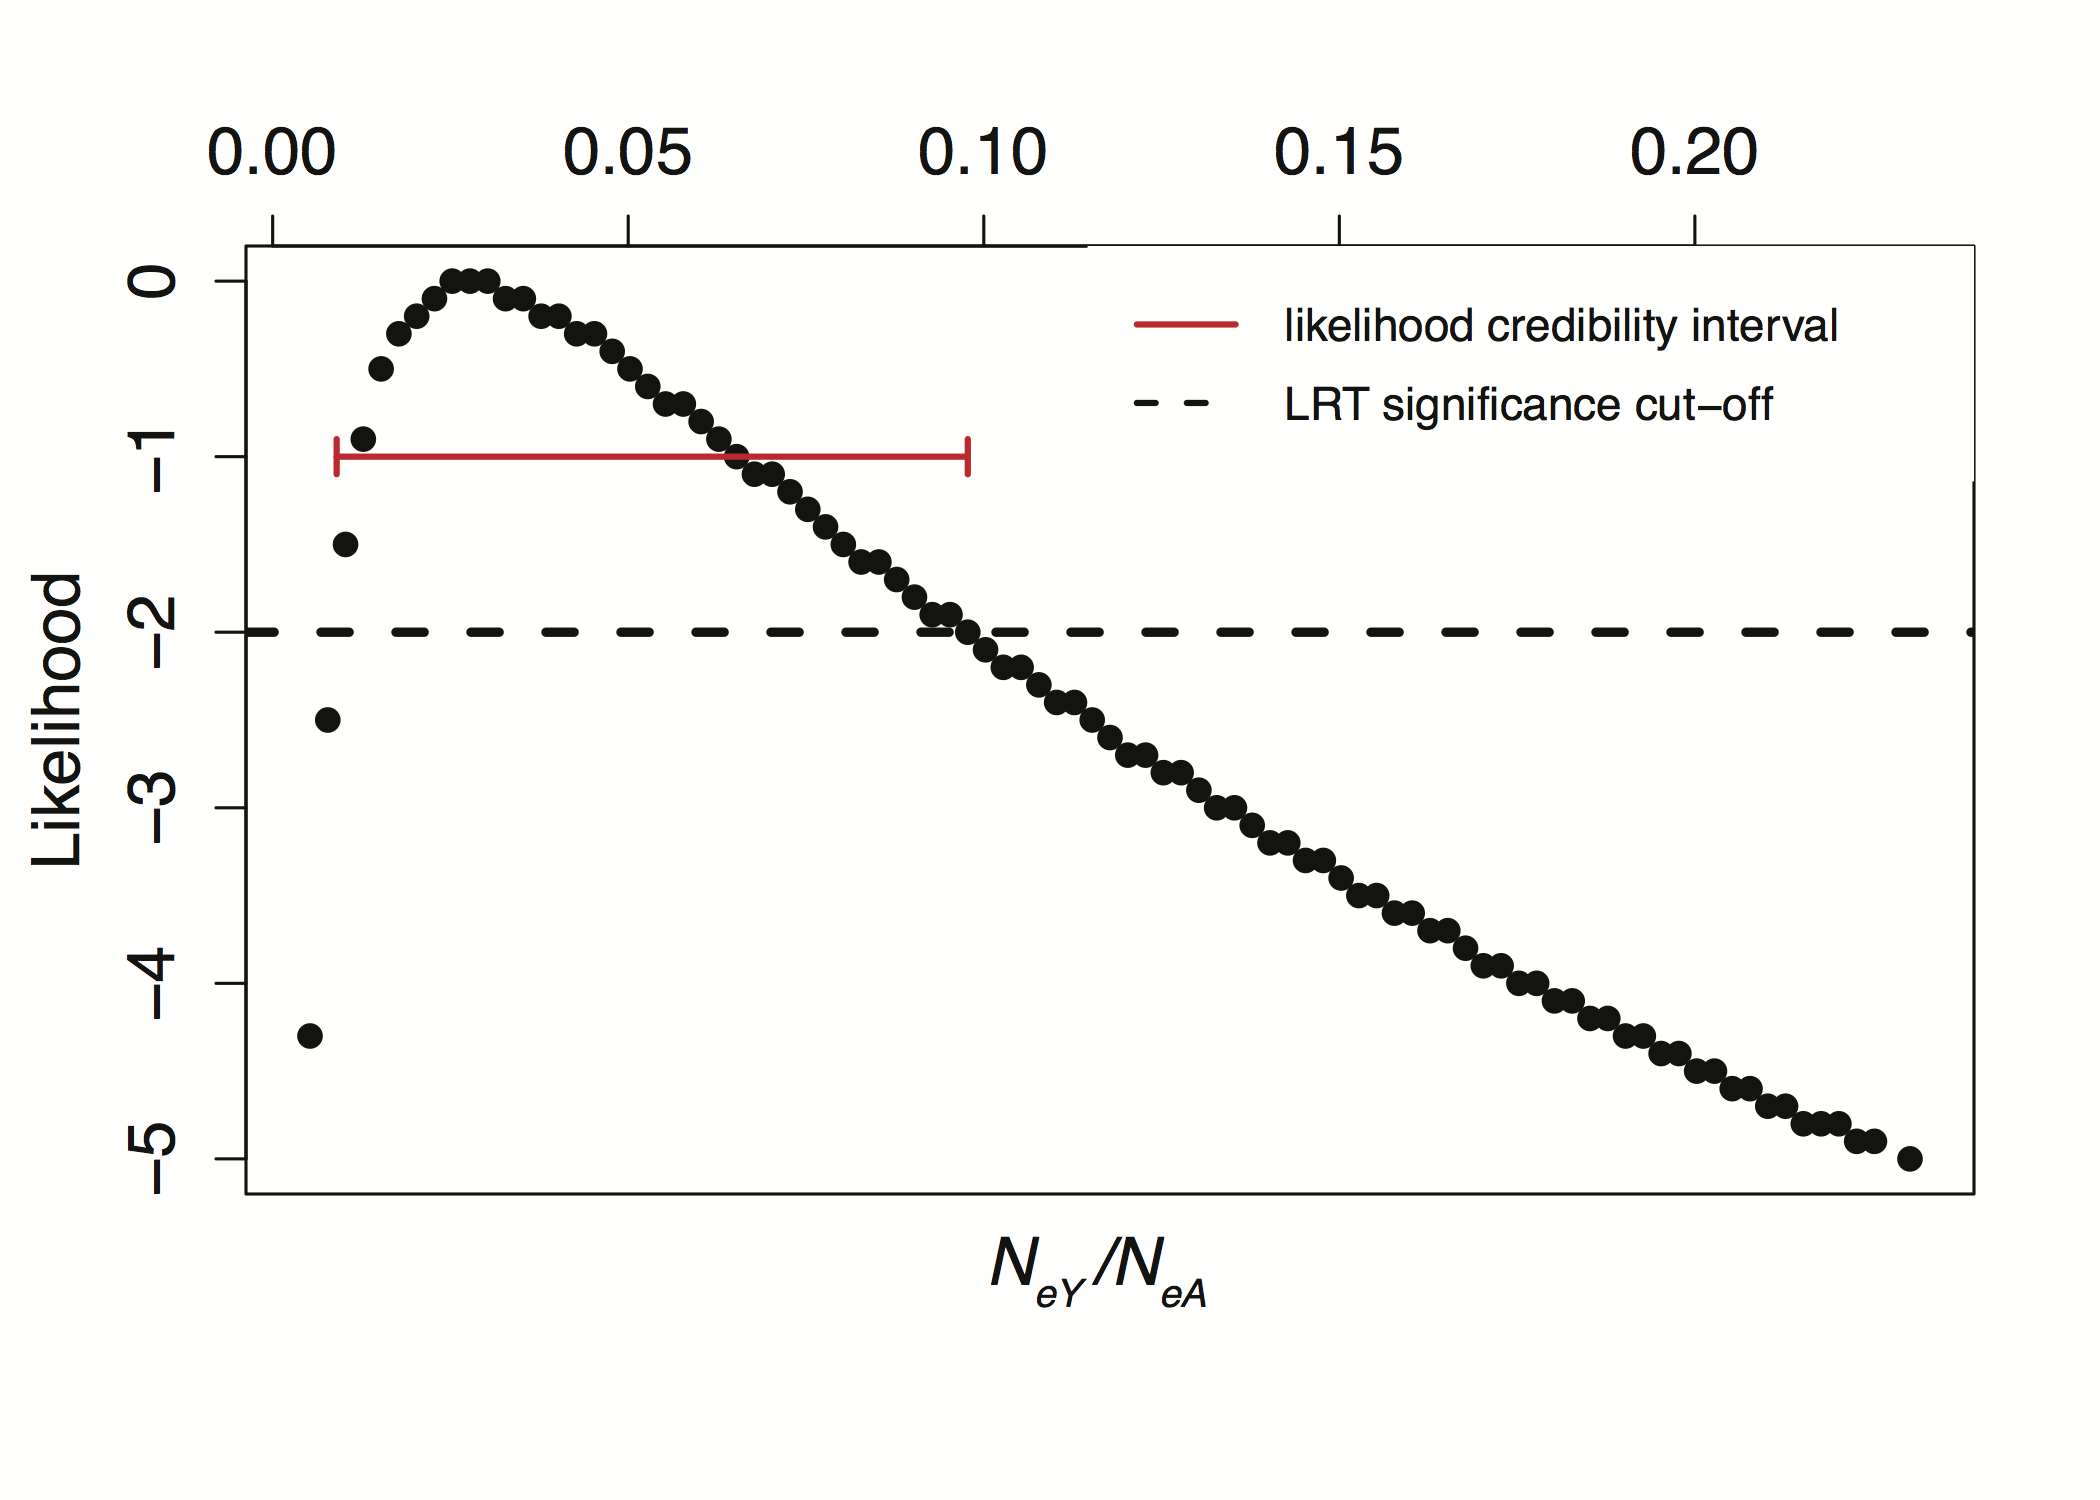
\includegraphics[width=.5\linewidth]{FigureS1.png}
\caption{likelihood estimation of the Y/A ratio}
\label{figure:FigureS1}
\end{figure}

%\begin{figure}[tbhp!]
%\centering
%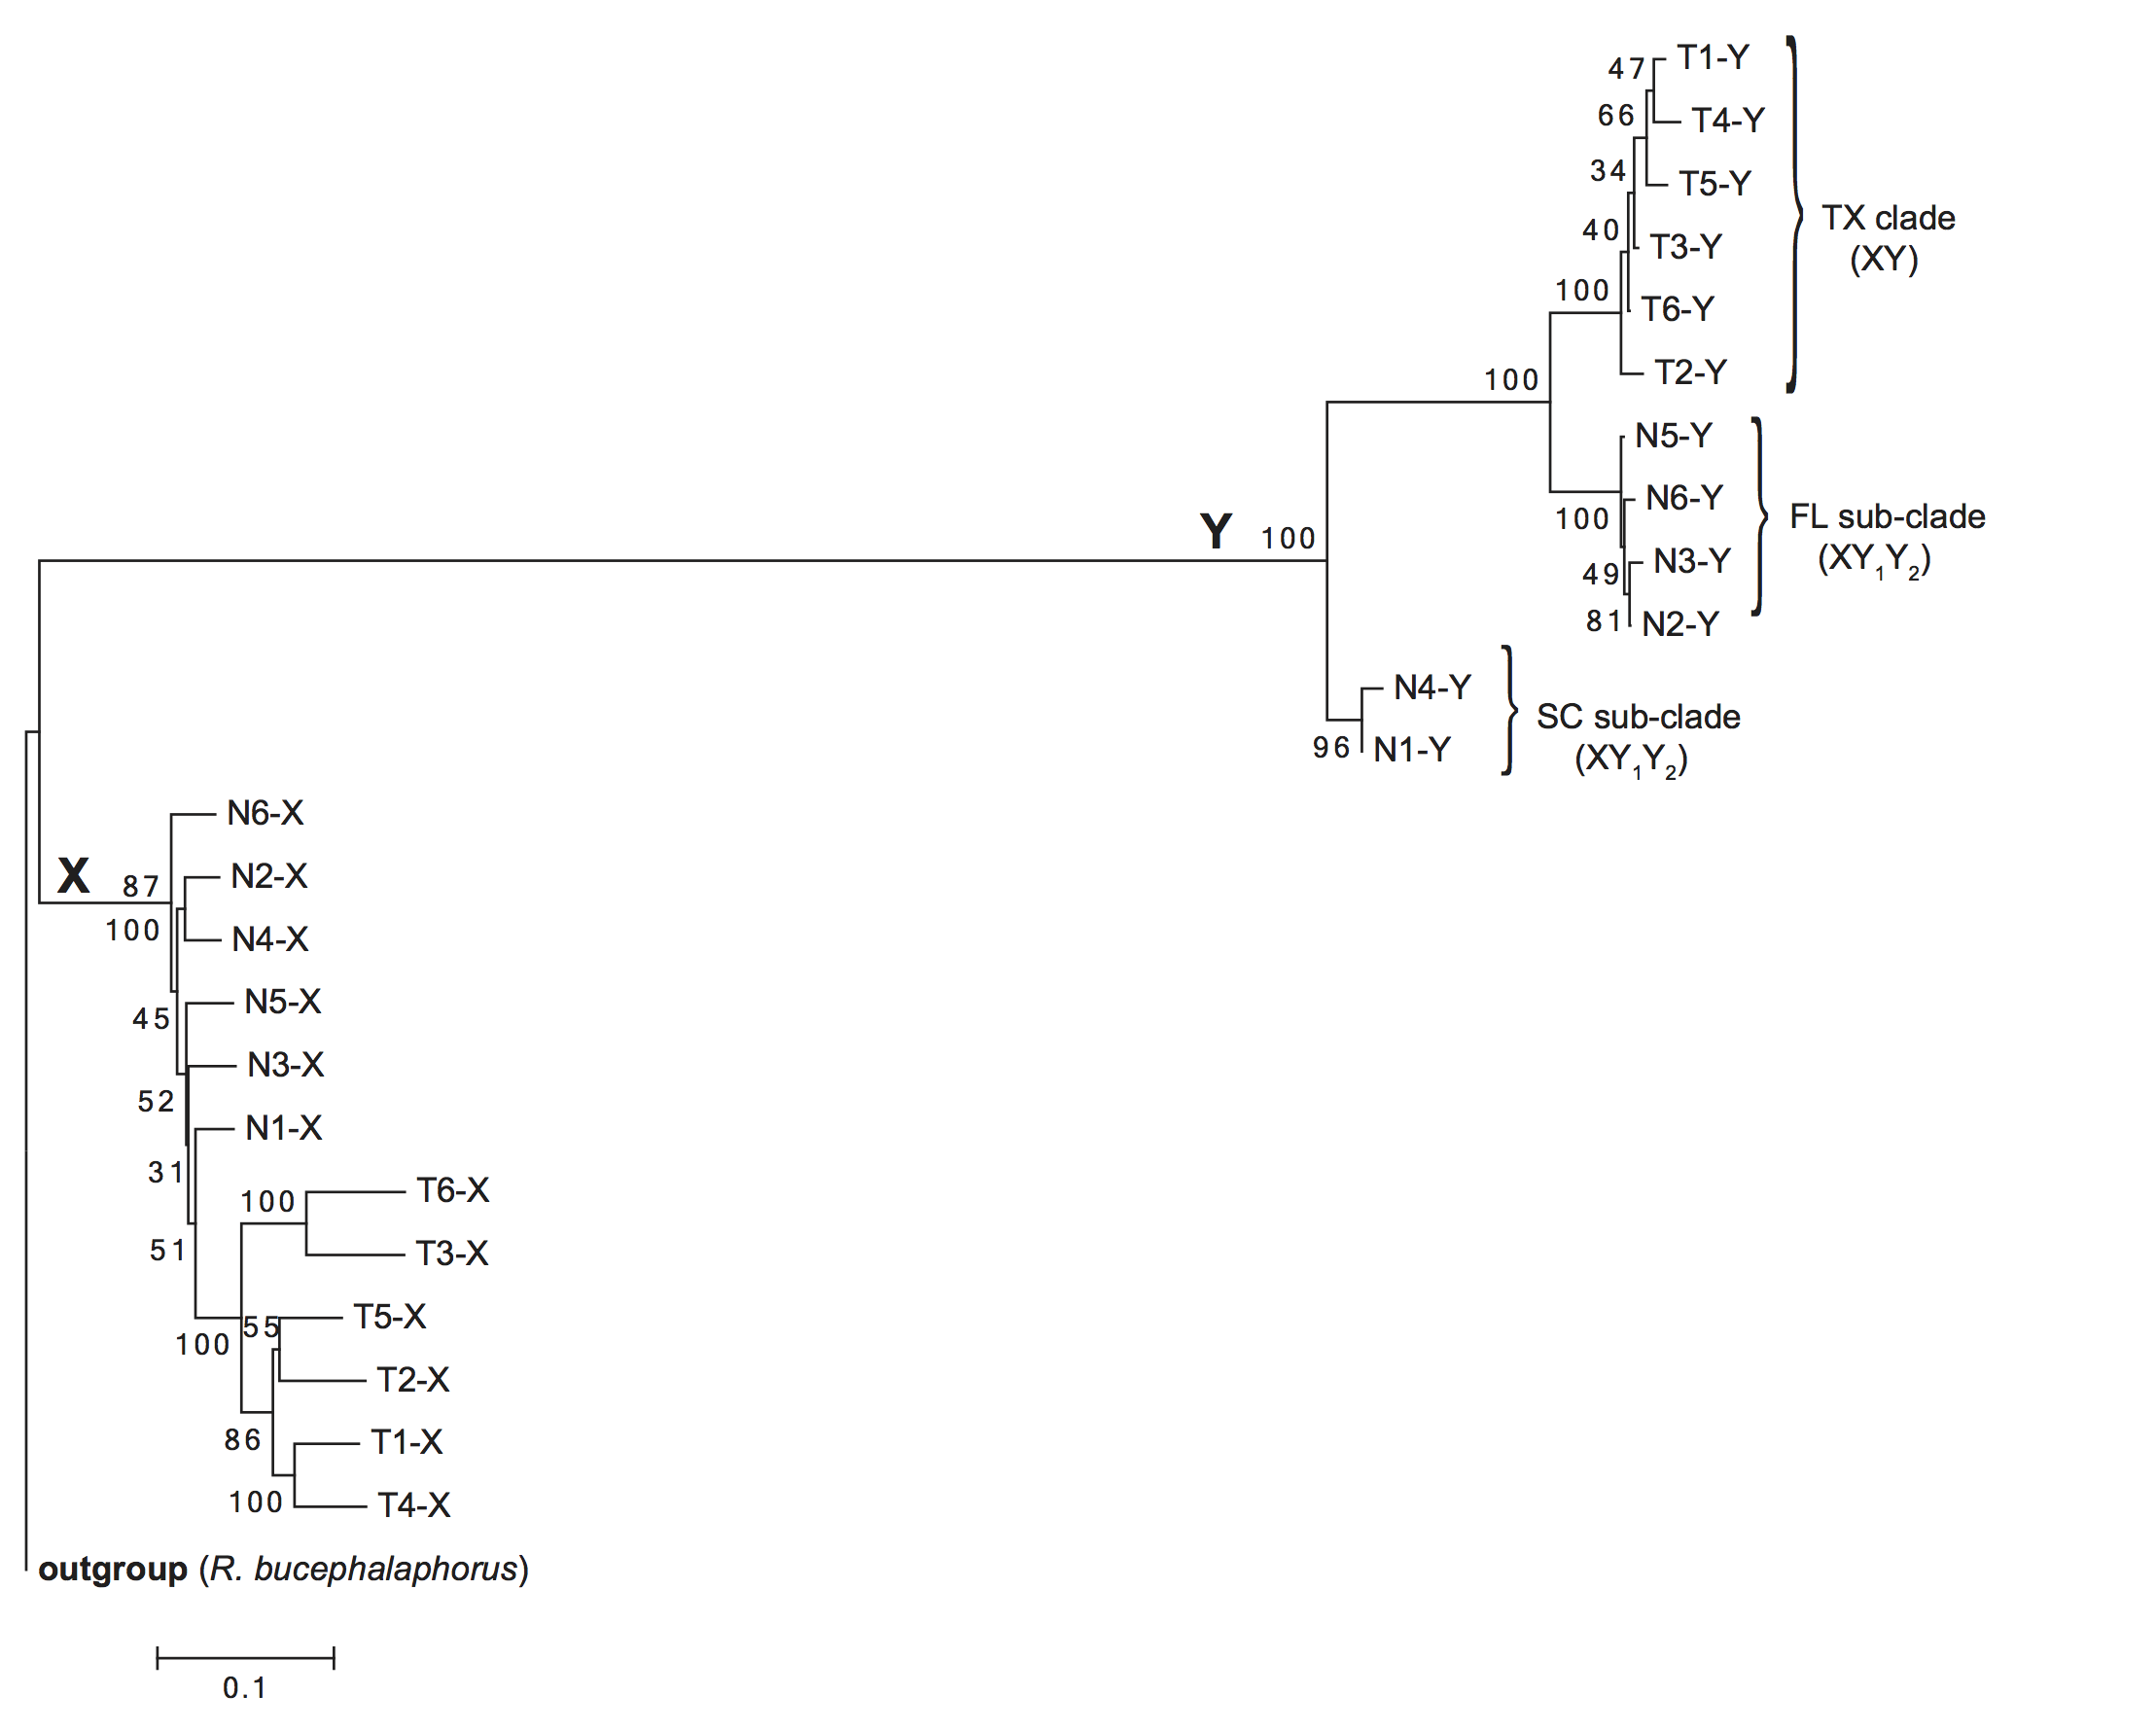
\includegraphics[width=.9\linewidth]{FigureS2.png}
%\caption{Evolutionary relationships of sex chromosome races in \textit{Rumex hastatulus}, inferred using the Neighbor-Joining method (Saitou and Nei 1987). The percentage of replicate trees in which the associated sequences clustered together in the bootstrap test (1000 replicates) is shown next to branches (Felsenstein 1985). The phylogeny is drawn to scale, with branch lengths in the same units as those of the evolutionary distances used to infer the tree. The evolutionary distances were computed using the Maximum Composite Likelihood method (Tamura et al. 2004) and are in the units of the number of base substitutions per site. The analysis was conducted on an alignment of X- and Y-linked genes from \textit{R. hastatulus}, with orthologous autosomal sequences from the non-dioecious but closely related outgroup species \textit{Rumex bucephalophorus} used to root the tree. ‘N’ designates the North Carolina race, and ‘T’ the Texas race, with numbers 1-6 corresponding to each of the 6 populations sampled. The inferred SC (South Carolina), and FL (Florida) sub-clades are indicated.}
%\label{figure:FigureS2}
%\end{figure}


%\begin{figure}[tbhp!]
%\centering
%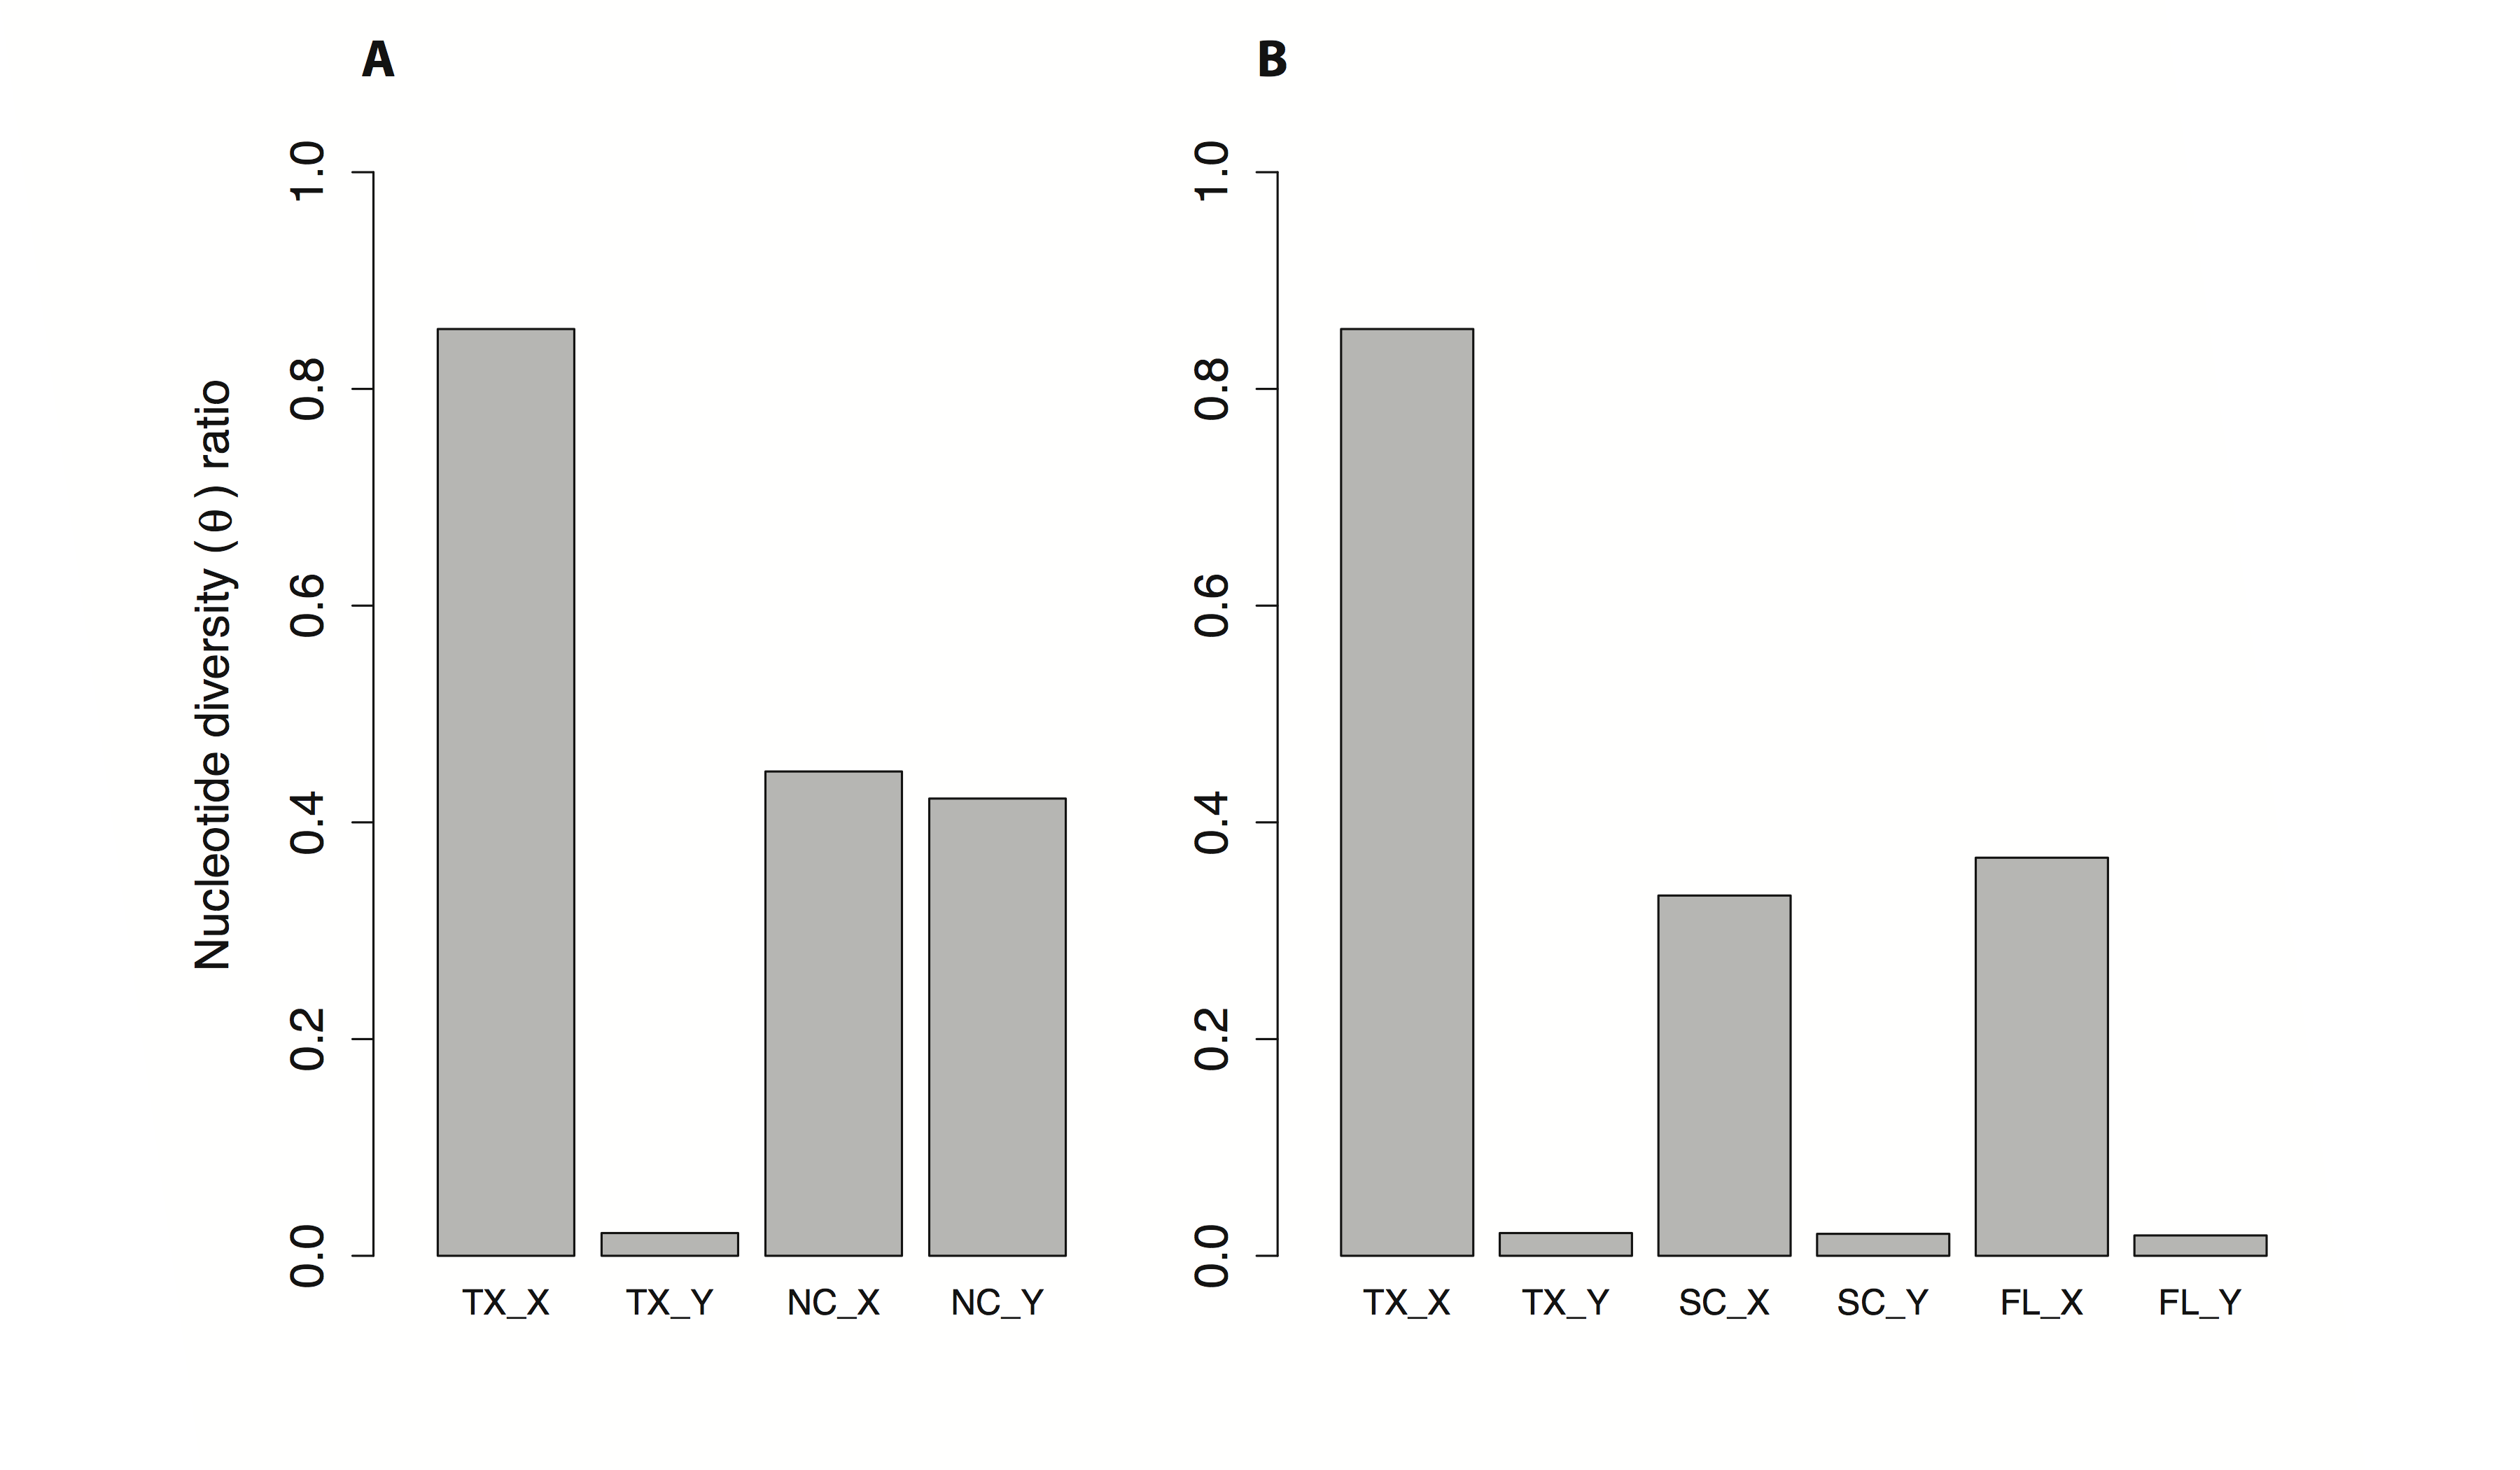
\includegraphics[width=1\linewidth]{FigureS3.png}
%\caption{Normalized X/A and Y/A nucleotide diversity ratios for XY and $XY_{1}Y_{2}$ races of \textit{Rumex hastatulus}. In \textbf{A}, the South Carolina and Florida sub-clades are collapsed into a single race (‘NC’), and in \textbf{B}, they are separated into the inferred ‘SC’ and ‘FL’ sub-clades.}
%\label{figure:FigureS3}
%\end{figure}


%Figure A4.1.2: Autosomal nucleotide diversity for the TX, SC, and FL clades of Rumex hastatulus, with confidence intervals calculated from bootstrapping 20000 replicates using the BCa method (Efron 1987) implemented in the Boot package in R (Canty and Ripley 2012; R Core Team 2011).

%\newpage
%\section*{Simulation code}

%\begin{lstlisting}
%#!/bin/bash

%#purifying selection
%sfs_code 1 50 -r 0 -t 0.001375 -P 1 -TE 0.3 -L 2 500000 800000 \
%-a N -W L 1 2 0 1 1 0.184 0.003 -n 8 -N 500 -A

%#positive selection
%sfs code 1 2000 -n 20 -N <N> -Td 0 -TE <> -W <type> [args]

%\end{lstlisting}

\end{document}